\headerbox{\bf\color{sufered} Experiments}
{name=experiments,column=2,span=3,below=update-rule}
{
    We evaluate the performance of the proposed
    SPLR algorithm via a series of numerical experiments, and compare SPLR with a number of widely-used algorithms for solving entropic-regularized OT.

    \begin{minipage}[c]{0.48\textwidth}
        \centering
        \vspace{0.5em}
        {\bf\color{sufered} Synthetic Data} \\ \vspace{0.3em}
        \includegraphics[width=0.3\textwidth]{save/Synthetic I/run_times/n=1000, m=1000, reg=0.001}
        \includegraphics[width=0.3\textwidth]{save/Synthetic I/run_times/n=5000, m=5000, reg=0.001}
        \includegraphics[width=0.3\textwidth]{save/Synthetic I/run_times/n=10000, m=10000, reg=0.001} \\
        \includegraphics[width=0.3\textwidth]{save/Synthetic II/run_times/n=1000, m=1000, reg=0.001}
        \includegraphics[width=0.3\textwidth]{save/Synthetic II/run_times/n=5000, m=5000, reg=0.001}
        \includegraphics[width=0.3\textwidth]{save/Synthetic II/run_times/n=10000, m=10000, reg=0.001} \\
        
    \end{minipage}
    \hfill
    \begin{minipage}[c]{0.48\textwidth}
        \centering
        \vspace{0.5em}
        {\bf\color{sufered} (Fashion-)MNIST} \\ \vspace{0.3em}
        \includegraphics[width=0.3\textwidth]{save/MNIST/run_times/ID1=2, ID2=54698, norm=l1, reg=0.001}
        \includegraphics[width=0.3\textwidth]{save/MNIST/run_times/ID1=239, ID2=43981, norm=l1, reg=0.001}
        \includegraphics[width=0.3\textwidth]{save/MNIST/run_times/ID1=17390, ID2=49947, norm=l1, reg=0.001} \\
        \includegraphics[width=0.3\textwidth]{save/Fashion-MNIST/run_times/ID1=2, ID2=54698, norm=l1, reg=0.001}
        \includegraphics[width=0.3\textwidth]{save/Fashion-MNIST/run_times/ID1=239, ID2=43981, norm=l1, reg=0.001}
        \includegraphics[width=0.3\textwidth]{save/Fashion-MNIST/run_times/ID1=17390, ID2=49947, norm=l1, reg=0.001}\\
    \end{minipage}

    \vspace{0.5em}

    \begin{minipage}[c]{0.48\textwidth}
        \centering
        \vspace{0.5em}
        {\bf\color{sufered} Imagenet} \\ \vspace{0.3em}
        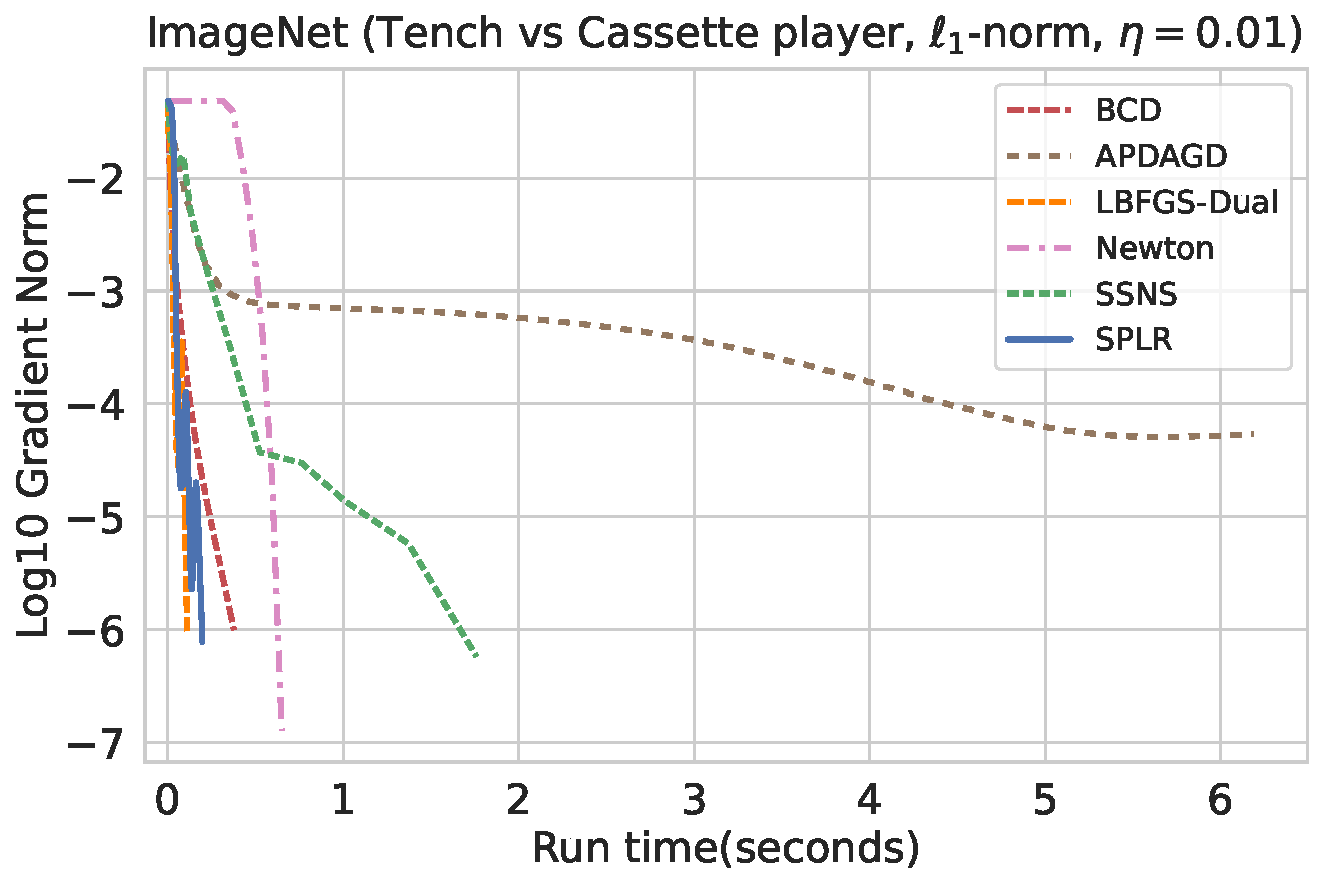
\includegraphics[width=0.3\textwidth]{save/ImageNet - Extra/run_times/CLASS1=tench, CLASS2=cassette player, dim=30, norm=l1, reg=0.01.pdf}
        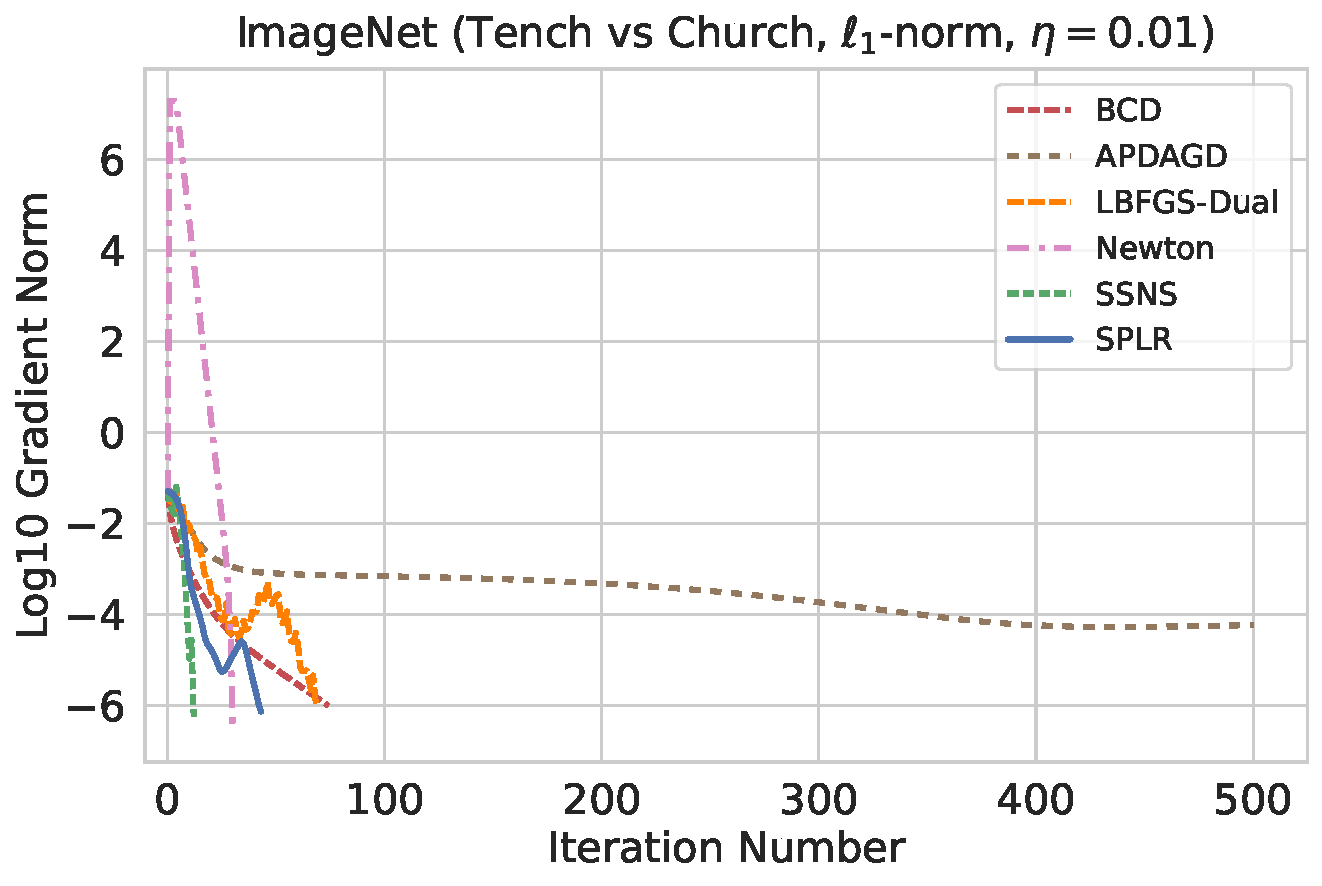
\includegraphics[width=0.3\textwidth]{save/ImageNet - Extra/run_times/CLASS1=tench, CLASS2=church, dim=30, norm=l1, reg=0.01.pdf}
        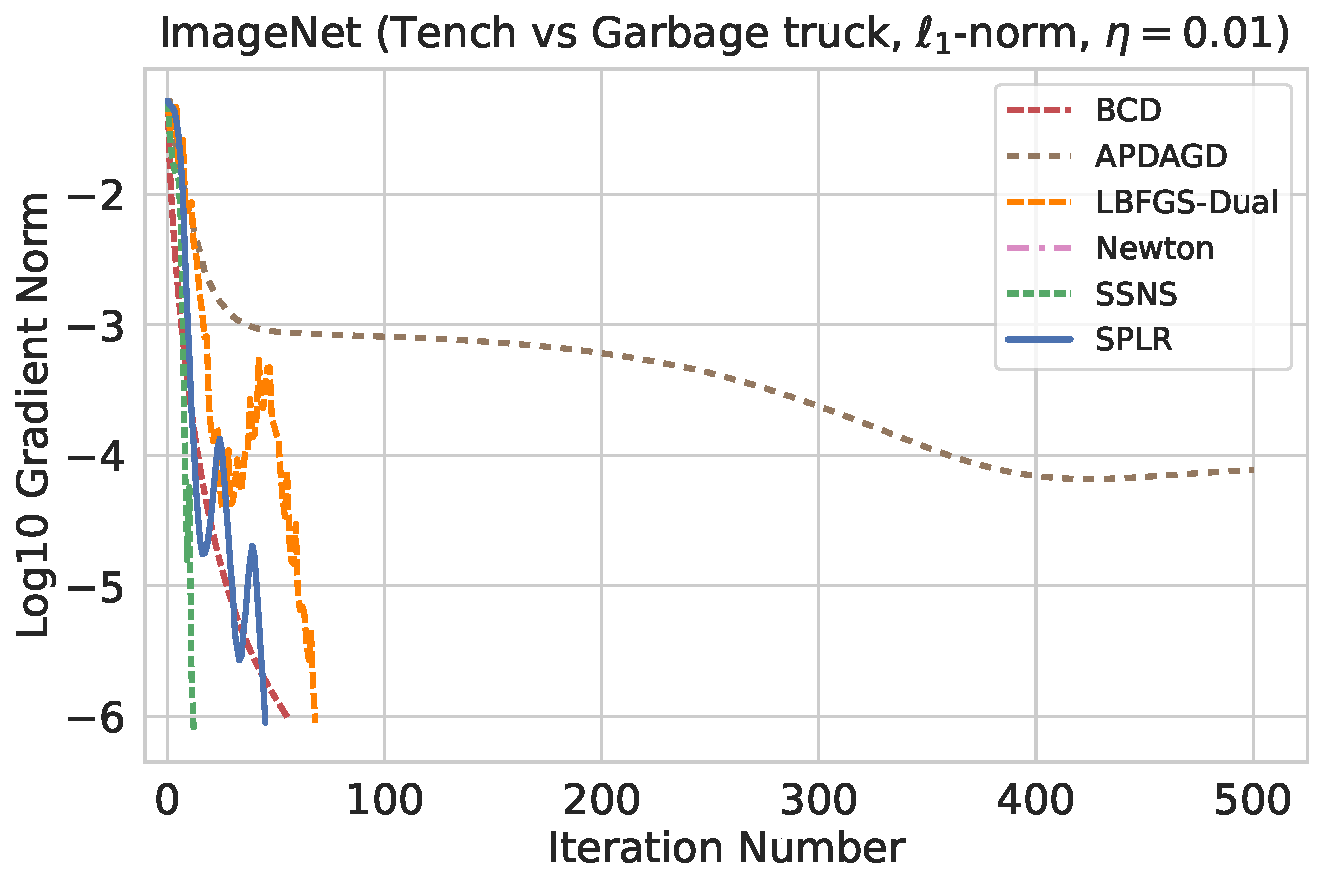
\includegraphics[width=0.3\textwidth]{save/ImageNet - Extra/run_times/CLASS1=tench, CLASS2=garbage truck, dim=30, norm=l1, reg=0.01.pdf} \\
        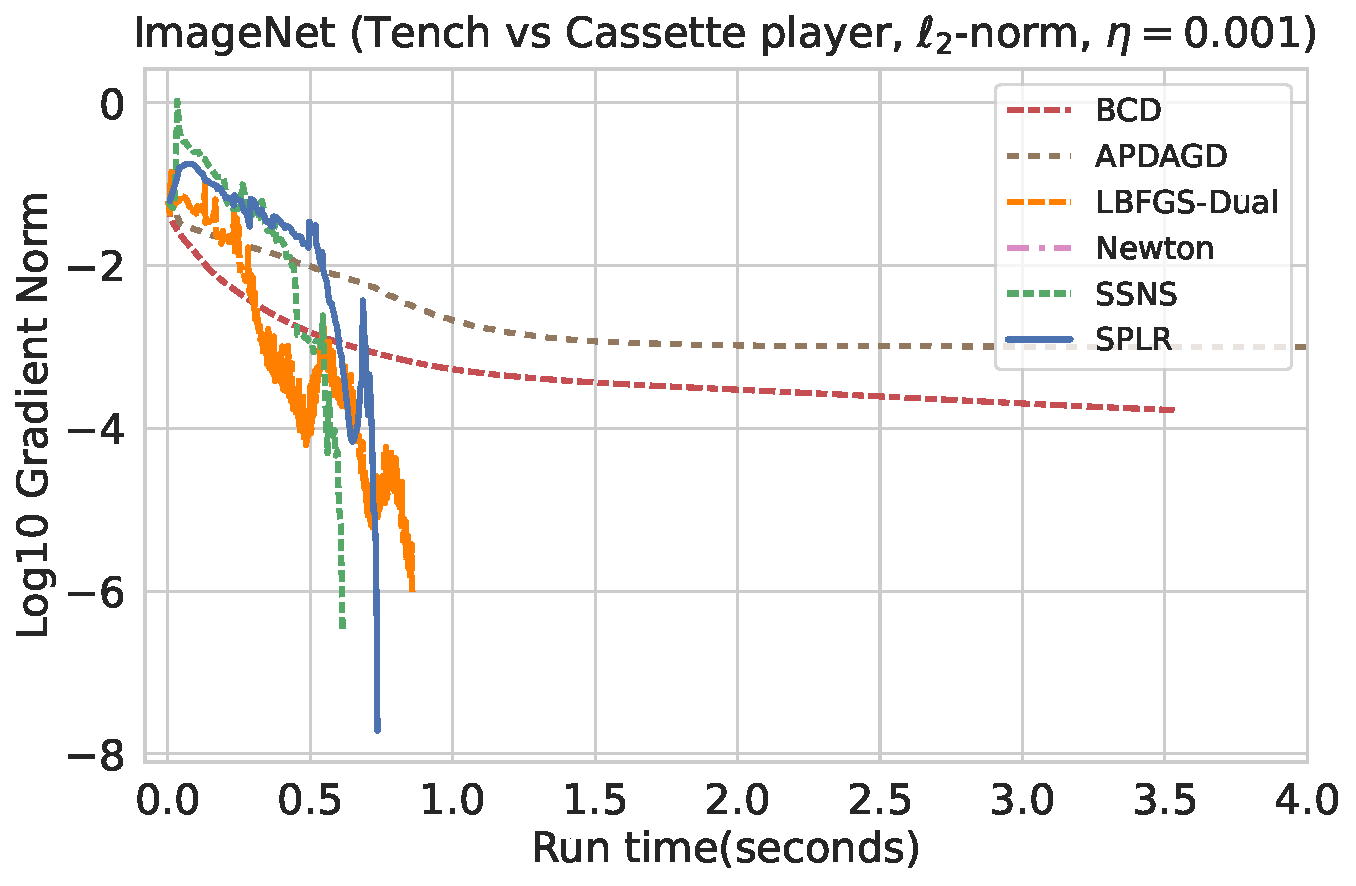
\includegraphics[width=0.3\textwidth]{save/ImageNet - Extra/run_times/CLASS1=tench, CLASS2=cassette player, dim=30, norm=l2, reg=0.001.pdf}
        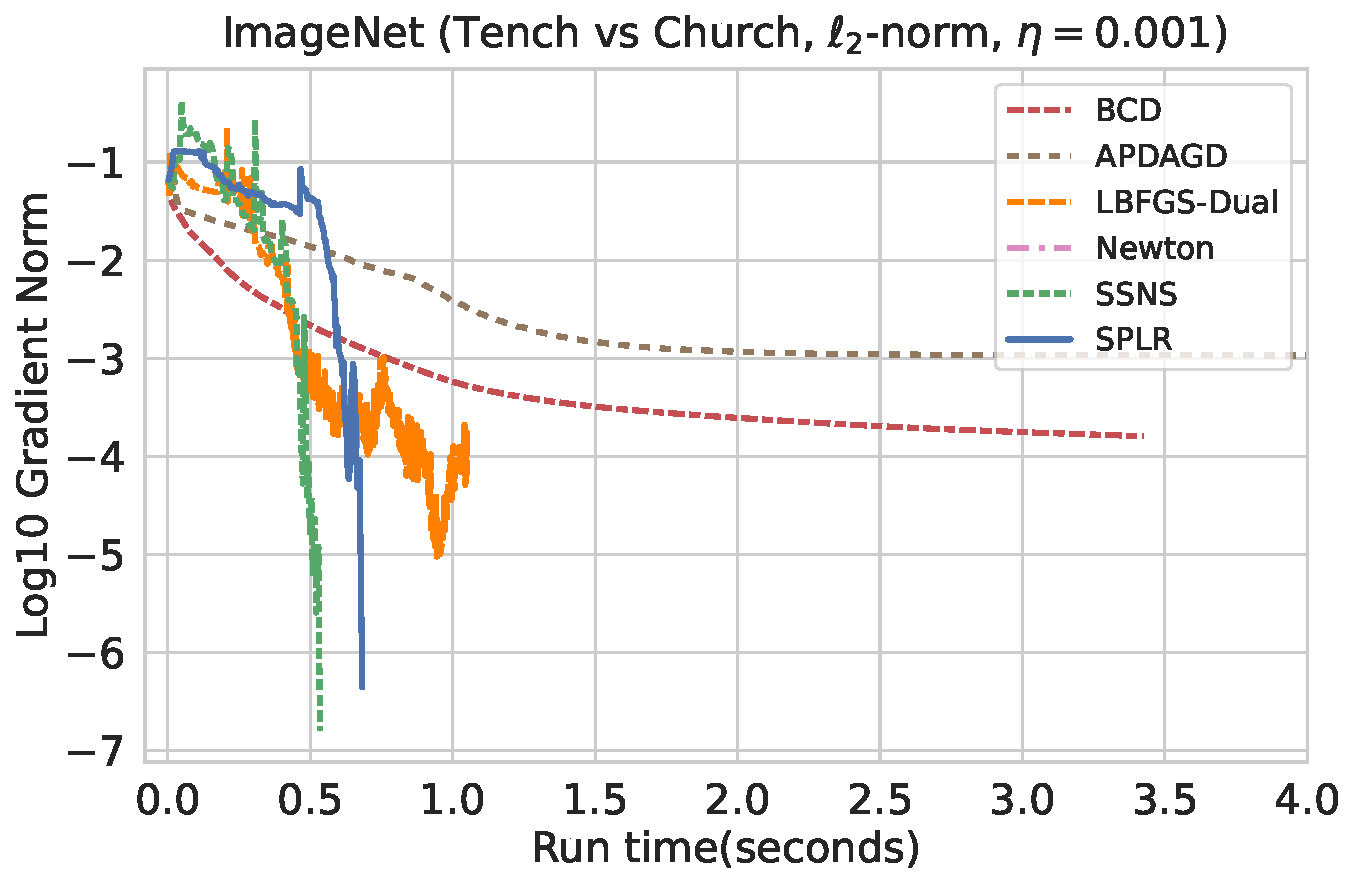
\includegraphics[width=0.3\textwidth]{save/ImageNet - Extra/run_times/CLASS1=tench, CLASS2=church, dim=30, norm=l2, reg=0.001.pdf}
        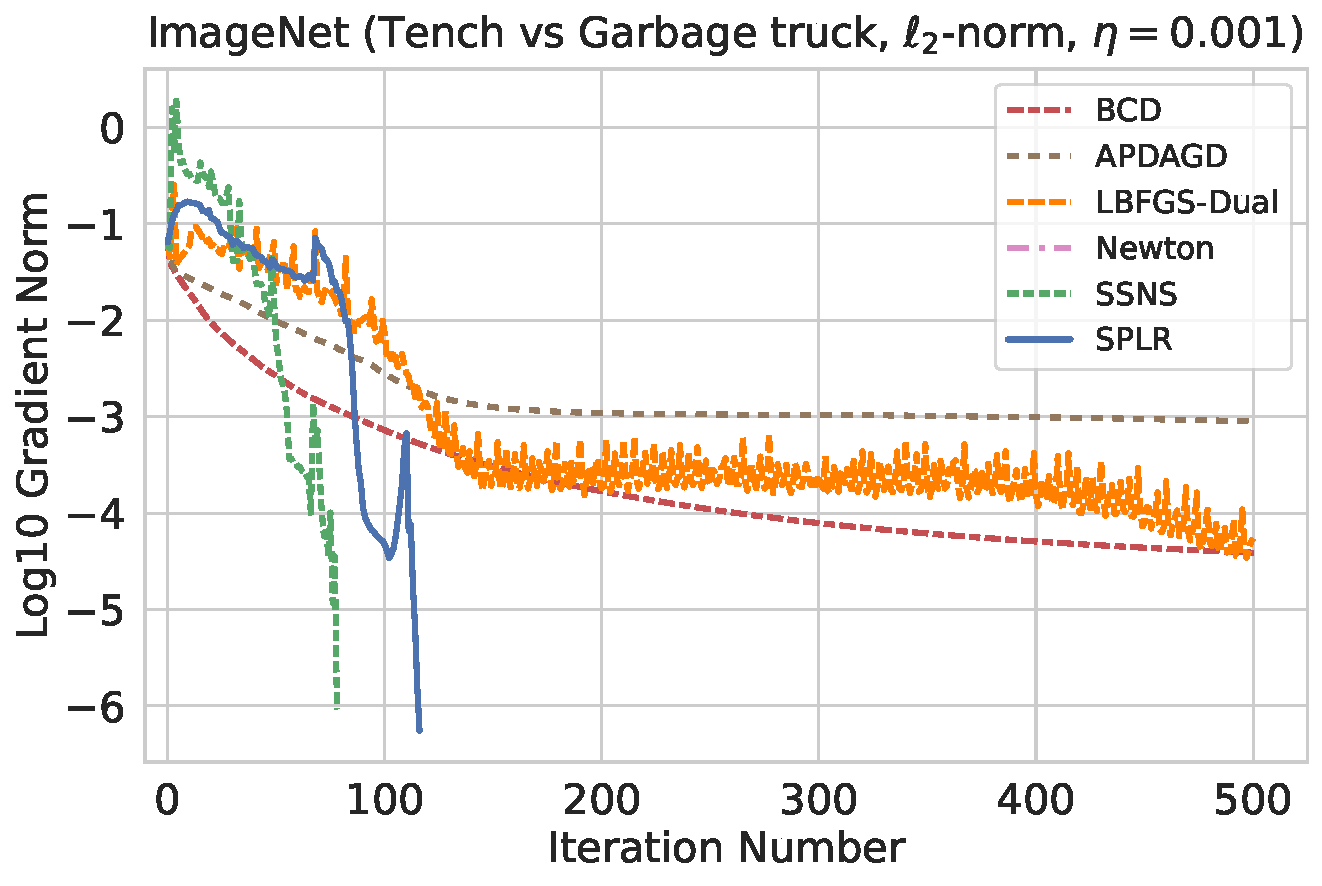
\includegraphics[width=0.3\textwidth]{save/ImageNet - Extra/run_times/CLASS1=tench, CLASS2=garbage truck, dim=30, norm=l2, reg=0.001.pdf} \\
    \end{minipage}
    \hfill
    \begin{minipage}[c]{0.48\textwidth}
        \centering
        \vspace{0.5em}
        {\bf\color{sufered} Effect of low-rank terms} \\ \vspace{0.3em}
        \includegraphics[width=0.3\textwidth]{save/Synthetic I - Ablation/run_times/n=1000, m=1000, reg=0.001.pdf}
        \includegraphics[width=0.3\textwidth]{save/Synthetic I - Ablation/run_times/n=5000, m=5000, reg=0.001.pdf}
        \includegraphics[width=0.3\textwidth]{save/Synthetic I - Ablation/run_times/n=10000, m=10000, reg=0.001.pdf} \\
        \includegraphics[width=0.3\textwidth]{save/Synthetic II - Ablation/run_times/n=1000, m=1000, reg=0.001.pdf}
        \includegraphics[width=0.3\textwidth]{save/Synthetic II - Ablation/run_times/n=5000, m=5000, reg=0.001.pdf}
        \includegraphics[width=0.3\textwidth]{save/Synthetic II - Ablation/run_times/n=10000, m=10000, reg=0.001.pdf} \\
    \end{minipage}

}